

\tikzset{every picture/.style={line width=0.75pt}} %set default line width to 0.75pt        

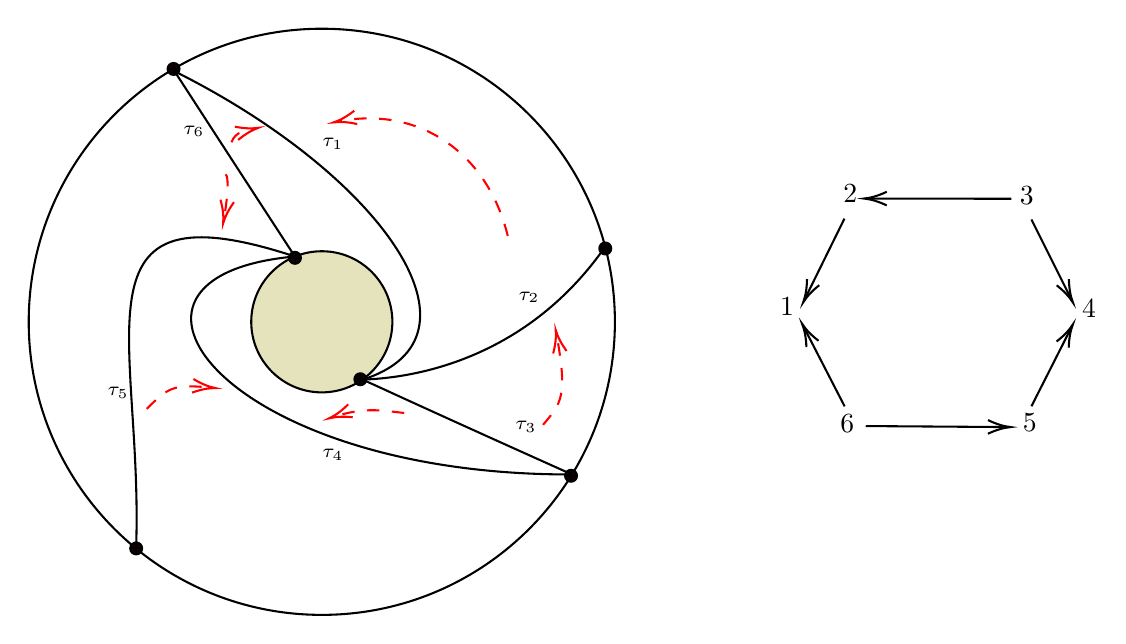
\begin{tikzpicture}[x=0.75pt,y=0.75pt,yscale=-1,xscale=1]
%uncomment if require: \path (0,458); %set diagram left start at 0, and has height of 458

%Shape: Circle [id:dp011167431945667827] 
\draw   (11,248.38) .. controls (11,170.39) and (74.22,107.17) .. (152.21,107.17) .. controls (230.2,107.17) and (293.42,170.39) .. (293.42,248.38) .. controls (293.42,326.36) and (230.2,389.58) .. (152.21,389.58) .. controls (74.22,389.58) and (11,326.36) .. (11,248.38) -- cycle ;
%Shape: Circle [id:dp7048127758853319] 
\draw  [fill={rgb, 255:red, 228; green, 227; blue, 188 }  ,fill opacity=1 ] (118.21,248.38) .. controls (118.21,229.6) and (133.43,214.38) .. (152.21,214.38) .. controls (170.99,214.38) and (186.21,229.6) .. (186.21,248.38) .. controls (186.21,267.15) and (170.99,282.38) .. (152.21,282.38) .. controls (133.43,282.38) and (118.21,267.15) .. (118.21,248.38) -- cycle ;
\draw  [fill={rgb, 255:red, 19; green, 1; blue, 1 }  ,fill opacity=1 ] (77.92,126.55) .. controls (77.92,124.97) and (79.2,123.69) .. (80.78,123.69) .. controls (82.36,123.69) and (83.64,124.97) .. (83.64,126.55) .. controls (83.64,128.13) and (82.36,129.42) .. (80.78,129.42) .. controls (79.2,129.42) and (77.92,128.13) .. (77.92,126.55) -- cycle ; \draw   (77.92,126.55) -- (83.64,126.55) ; \draw   (80.78,123.69) -- (80.78,129.42) ;
\draw  [fill={rgb, 255:red, 19; green, 1; blue, 1 }  ,fill opacity=1 ] (59.92,357.55) .. controls (59.92,355.97) and (61.2,354.69) .. (62.78,354.69) .. controls (64.36,354.69) and (65.64,355.97) .. (65.64,357.55) .. controls (65.64,359.13) and (64.36,360.42) .. (62.78,360.42) .. controls (61.2,360.42) and (59.92,359.13) .. (59.92,357.55) -- cycle ; \draw   (59.92,357.55) -- (65.64,357.55) ; \draw   (62.78,354.69) -- (62.78,360.42) ;
\draw  [fill={rgb, 255:red, 19; green, 1; blue, 1 }  ,fill opacity=1 ] (136.42,217.55) .. controls (136.42,215.97) and (137.7,214.69) .. (139.28,214.69) .. controls (140.86,214.69) and (142.14,215.97) .. (142.14,217.55) .. controls (142.14,219.13) and (140.86,220.42) .. (139.28,220.42) .. controls (137.7,220.42) and (136.42,219.13) .. (136.42,217.55) -- cycle ; \draw   (136.42,217.55) -- (142.14,217.55) ; \draw   (139.28,214.69) -- (139.28,220.42) ;
\draw  [fill={rgb, 255:red, 19; green, 1; blue, 1 }  ,fill opacity=1 ] (167.92,276.05) .. controls (167.92,274.47) and (169.2,273.19) .. (170.78,273.19) .. controls (172.36,273.19) and (173.64,274.47) .. (173.64,276.05) .. controls (173.64,277.63) and (172.36,278.92) .. (170.78,278.92) .. controls (169.2,278.92) and (167.92,277.63) .. (167.92,276.05) -- cycle ; \draw   (167.92,276.05) -- (173.64,276.05) ; \draw   (170.78,273.19) -- (170.78,278.92) ;
\draw  [fill={rgb, 255:red, 19; green, 1; blue, 1 }  ,fill opacity=1 ] (269.42,322.55) .. controls (269.42,320.97) and (270.7,319.69) .. (272.28,319.69) .. controls (273.86,319.69) and (275.14,320.97) .. (275.14,322.55) .. controls (275.14,324.13) and (273.86,325.42) .. (272.28,325.42) .. controls (270.7,325.42) and (269.42,324.13) .. (269.42,322.55) -- cycle ; \draw   (269.42,322.55) -- (275.14,322.55) ; \draw   (272.28,319.69) -- (272.28,325.42) ;
\draw  [fill={rgb, 255:red, 19; green, 1; blue, 1 }  ,fill opacity=1 ] (285.92,213.05) .. controls (285.92,211.47) and (287.2,210.19) .. (288.78,210.19) .. controls (290.36,210.19) and (291.64,211.47) .. (291.64,213.05) .. controls (291.64,214.63) and (290.36,215.92) .. (288.78,215.92) .. controls (287.2,215.92) and (285.92,214.63) .. (285.92,213.05) -- cycle ; \draw   (285.92,213.05) -- (291.64,213.05) ; \draw   (288.78,210.19) -- (288.78,215.92) ;
%Curve Lines [id:da8637706579523565] 
\draw    (80.75,127.42) .. controls (80.75,126.42) and (81.25,127.92) .. (139.25,216.92) ;
%Curve Lines [id:da8931038200838086] 
\draw    (80.75,127.42) .. controls (181.25,177.42) and (236.75,256.42) .. (171.25,276.42) ;
%Curve Lines [id:da4496396466165504] 
\draw    (171.25,276.42) .. controls (171.25,275.42) and (171.25,276.42) .. (272.75,321.92) ;
%Curve Lines [id:da8914629129152412] 
\draw    (171.25,276.42) .. controls (171.25,275.42) and (241.25,279.42) .. (288.25,212.92) ;
%Curve Lines [id:da9415141411706016] 
\draw    (139.25,216.92) .. controls (32.75,226.42) and (105.25,322.42) .. (272.75,321.92) ;
%Curve Lines [id:da7175871064348958] 
\draw    (139.25,216.92) .. controls (28.75,180.5) and (66.25,256.5) .. (62.75,357) ;
%Straight Lines [id:da08883384268274452] 
\draw    (415.47,189) -- (484.4,189.1) ;
\draw [shift={(413.47,189)}, rotate = 0.08] [color={rgb, 255:red, 0; green, 0; blue, 0 }  ][line width=0.75]    (10.93,-3.29) .. controls (6.95,-1.4) and (3.31,-0.3) .. (0,0) .. controls (3.31,0.3) and (6.95,1.4) .. (10.93,3.29)   ;
%Straight Lines [id:da8222561468381305] 
\draw    (384.98,237.31) -- (404,198.7) ;
\draw [shift={(384.1,239.1)}, rotate = 296.22] [color={rgb, 255:red, 0; green, 0; blue, 0 }  ][line width=0.75]    (10.93,-3.29) .. controls (6.95,-1.4) and (3.31,-0.3) .. (0,0) .. controls (3.31,0.3) and (6.95,1.4) .. (10.93,3.29)   ;
%Straight Lines [id:da4094285868006836] 
\draw    (482.1,299.09) -- (414.28,298.61) ;
\draw [shift={(484.1,299.1)}, rotate = 180.4] [color={rgb, 255:red, 0; green, 0; blue, 0 }  ][line width=0.75]    (10.93,-3.29) .. controls (6.95,-1.4) and (3.31,-0.3) .. (0,0) .. controls (3.31,0.3) and (6.95,1.4) .. (10.93,3.29)   ;
%Straight Lines [id:da646049799635397] 
\draw    (404.1,289.1) -- (384.52,251.08) ;
\draw [shift={(383.6,249.3)}, rotate = 62.75] [color={rgb, 255:red, 0; green, 0; blue, 0 }  ][line width=0.75]    (10.93,-3.29) .. controls (6.95,-1.4) and (3.31,-0.3) .. (0,0) .. controls (3.31,0.3) and (6.95,1.4) .. (10.93,3.29)   ;
%Straight Lines [id:da7199087896373981] 
\draw    (494.1,199.1) -- (513.21,237.31) ;
\draw [shift={(514.1,239.1)}, rotate = 243.43] [color={rgb, 255:red, 0; green, 0; blue, 0 }  ][line width=0.75]    (10.93,-3.29) .. controls (6.95,-1.4) and (3.31,-0.3) .. (0,0) .. controls (3.31,0.3) and (6.95,1.4) .. (10.93,3.29)   ;
%Straight Lines [id:da2644151150412464] 
\draw    (513.2,251.38) -- (494.1,289.1) ;
\draw [shift={(514.1,249.6)}, rotate = 116.85] [color={rgb, 255:red, 0; green, 0; blue, 0 }  ][line width=0.75]    (10.93,-3.29) .. controls (6.95,-1.4) and (3.31,-0.3) .. (0,0) .. controls (3.31,0.3) and (6.95,1.4) .. (10.93,3.29)   ;
%Curve Lines [id:da3563655424763953] 
\draw [color={rgb, 255:red, 255; green, 0; blue, 0 }  ,draw opacity=1 ] [dash pattern={on 4.5pt off 4.5pt}]  (241.8,207) .. controls (232.05,166.91) and (198.91,143.99) .. (159.7,151.92) ;
\draw [shift={(157.9,152.3)}, rotate = 347.32] [color={rgb, 255:red, 255; green, 0; blue, 0 }  ,draw opacity=1 ][line width=0.75]    (10.93,-3.29) .. controls (6.95,-1.4) and (3.31,-0.3) .. (0,0) .. controls (3.31,0.3) and (6.95,1.4) .. (10.93,3.29)   ;
%Curve Lines [id:da8508534327134905] 
\draw [color={rgb, 255:red, 255; green, 0; blue, 0 }  ,draw opacity=1 ] [dash pattern={on 4.5pt off 4.5pt}]  (191.9,292.3) .. controls (182.25,291.34) and (173.34,289.07) .. (157.46,294.3) ;
\draw [shift={(155.7,294.9)}, rotate = 340.56] [color={rgb, 255:red, 255; green, 0; blue, 0 }  ,draw opacity=1 ][line width=0.75]    (10.93,-3.29) .. controls (6.95,-1.4) and (3.31,-0.3) .. (0,0) .. controls (3.31,0.3) and (6.95,1.4) .. (10.93,3.29)   ;
%Curve Lines [id:da2595129660274895] 
\draw [color={rgb, 255:red, 255; green, 0; blue, 0 }  ,draw opacity=1 ] [dash pattern={on 4.5pt off 4.5pt}]  (258.8,298) .. controls (267.72,287.51) and (270.78,284.42) .. (265.25,254.19) ;
\draw [shift={(264.9,252.3)}, rotate = 79.38] [color={rgb, 255:red, 255; green, 0; blue, 0 }  ,draw opacity=1 ][line width=0.75]    (10.93,-3.29) .. controls (6.95,-1.4) and (3.31,-0.3) .. (0,0) .. controls (3.31,0.3) and (6.95,1.4) .. (10.93,3.29)   ;
%Curve Lines [id:da3406149837992146] 
\draw [color={rgb, 255:red, 255; green, 0; blue, 0 }  ,draw opacity=1 ] [dash pattern={on 4.5pt off 4.5pt}]  (67.9,290.3) .. controls (78.57,279.63) and (80.77,278.37) .. (99.15,280.13) ;
\draw [shift={(100.9,280.3)}, rotate = 185.71] [color={rgb, 255:red, 255; green, 0; blue, 0 }  ,draw opacity=1 ][line width=0.75]    (10.93,-3.29) .. controls (6.95,-1.4) and (3.31,-0.3) .. (0,0) .. controls (3.31,0.3) and (6.95,1.4) .. (10.93,3.29)   ;
%Curve Lines [id:da24051616191269032] 
\draw [color={rgb, 255:red, 255; green, 0; blue, 0 }  ,draw opacity=1 ] [dash pattern={on 4.5pt off 4.5pt}]  (108.7,161.9) .. controls (110.41,156.77) and (115.78,156.03) .. (119.8,155.29) ;
\draw [shift={(121.7,154.9)}, rotate = 165.96] [color={rgb, 255:red, 255; green, 0; blue, 0 }  ,draw opacity=1 ][line width=0.75]    (10.93,-3.29) .. controls (6.95,-1.4) and (3.31,-0.3) .. (0,0) .. controls (3.31,0.3) and (6.95,1.4) .. (10.93,3.29)   ;
%Curve Lines [id:da5474461226079983] 
\draw [color={rgb, 255:red, 255; green, 0; blue, 0 }  ,draw opacity=1 ] [dash pattern={on 4.5pt off 4.5pt}]  (105.9,177.3) .. controls (107.6,178.81) and (106.8,188.72) .. (105.02,199.09) ;
\draw [shift={(104.7,200.9)}, rotate = 280.3] [color={rgb, 255:red, 255; green, 0; blue, 0 }  ,draw opacity=1 ][line width=0.75]    (10.93,-3.29) .. controls (6.95,-1.4) and (3.31,-0.3) .. (0,0) .. controls (3.31,0.3) and (6.95,1.4) .. (10.93,3.29)   ;

% Text Node
\draw (151,158.4) node [anchor=north west][inner sep=0.75pt]  [font=\scriptsize]  {$\tau _{1}$};
% Text Node
\draw (245.5,232.4) node [anchor=north west][inner sep=0.75pt]  [font=\scriptsize]  {$\tau _{2}$};
% Text Node
\draw (244,294.9) node [anchor=north west][inner sep=0.75pt]  [font=\scriptsize]  {$\tau _{3}$};
% Text Node
\draw (151,308.4) node [anchor=north west][inner sep=0.75pt]  [font=\scriptsize]  {$\tau _{4}$};
% Text Node
\draw (47.5,278.4) node [anchor=north west][inner sep=0.75pt]  [font=\scriptsize]  {$\tau _{5}$};
% Text Node
\draw (84,152.4) node [anchor=north west][inner sep=0.75pt]  [font=\scriptsize]  {$\tau _{6}$};
% Text Node
\draw (371.5,235.3) node [anchor=north west][inner sep=0.75pt]    {$1$};
% Text Node
\draw (402,180.8) node [anchor=north west][inner sep=0.75pt]    {$2$};
% Text Node
\draw (487,181.8) node [anchor=north west][inner sep=0.75pt]    {$3$};
% Text Node
\draw (517,236.3) node [anchor=north west][inner sep=0.75pt]    {$4$};
% Text Node
\draw (488.5,291.3) node [anchor=north west][inner sep=0.75pt]    {$5$};
% Text Node
\draw (400.5,291.8) node [anchor=north west][inner sep=0.75pt]    {$6$};


\end{tikzpicture}
